% Capitulo 5

\chapter{Análisis General} % Main chapter title

\label{AnalisisGeneral} % For referencing the chapter elsewhere, use \ref{Chapter1} 

\lhead{Capítulo 5 \emph{Análisis General}} % This is for the header on each page - perhaps a shortened title

El análisis es una etapa del desarrollo de software que tiene como finalidad ayudar al desarrollador a entender los deseos del cliente, delimitar la funcionalidad del sistema y analizar la factibilidad del mismo, para poder brindar una solución total al problema presentado.

\section{Estudio de Factibilidad}

\newcommand{\tabitem}{~~\llap{\textbullet}~~}

El estudio de factibilidad sirve para estimar los recursos necesarios para el desarrollo del proyecto, el éxito de la implementación está determinado por el grado de factibilidad que se presente en tres aspectos a evaluar: técnico, económico y operativo.

\subsection{Factibilidad Técnica}

La factibilidad técnica consiste en realizar una evaluación de la tecnología con la que cuenta el equipo de trabajo, en éste estudio se muestra la información recolectada sobre los componentes técnicos con los que se cuenta y la posibilidad de hacer uso de los mismos en el desarrollo e implementación del sistema propuesto y de ser necesario, los requisitos tecnológicos que deben ser adquiridos para el desarrollo y puesta en marcha del sistema. 

De acuerdo a los requisitos del sistema se evaluaron sus componentes bajo dos enfoques: hardware y software. 

\subsubsection{Hardware}

Respecto al hardware, se requieren equipos de cómputo para: desarrollar la aplicación móvil, alojar la aplicación Web de administración y tener el servicio Web funcionando. También es necesario un teléfono inteligente que cuente con los sensores necesarios para la localización en interiores. 

El equipo de trabajo cuenta con las computadoras personales para el desarrollo de la aplicación móvil, las cuales se detallan en la Tabla \ref{tab:hardware}.

\begin{table}[h]
	\begin{center}
		\begin{tabular}{|c|c|}
			\hline \rowcolor[RGB]{51,153,255}
			\textcolor{blanco}{\bf Recurso} &
				\textcolor{blanco}{\bf Características} \\
			\hline 
			\multirow{1}{2.8cm}{Laptop Lenovo} &
				{\parbox{0.5\textwidth}{
					\begin{itemize}
                			\item Procesador Intel Core i3 2.2 GHz
		               	\item 4 GB memoria RAM DDR3
                			\item 520 GB de disco duro
                			\item Sistema Operativo Windows 7 de 64 bits
           			\end{itemize} }} \\
      		\hline \rowcolor[RGB]{240,248,255} 
      		\multirow{1}{2.8cm}{MacBook Pro} &
      				{\parbox{0.5\textwidth}{
					\begin{itemize}
                			\item Procesador Intel Core i7 2.3 GHz
		               	\item 8 GB memoria RAM
                			\item 250 GB de almacenamiento en flash
                			\item Sistema Operativo OS X 10.10.1
           			\end{itemize} }} \\
      		\hline 
		\end{tabular}
	\end{center}
	\caption[Recursos de Hardware del Equipo]{Recursos de Hardware del Equipo} 
	\label{tab:hardware}
\end{table}

Debido a la naturaleza del sistema a desarrollar, se requiere de ciertos dispositivos móviles con las características necesarias para poder implementar y elaborar las pruebas necesarias a la aplicación móvil. En la Tabla \ref{tab:reqMin} se enlistan las características mínimas requeridas en dichos dispositivos móviles para el correcto funcionamiento de la aplicación.

\begin{table}[h]
	\begin{center}
		\begin{tabular}{|>{\columncolor[RGB]{51,153,255}}l|l|}
			\hline  
			\textcolor{blanco}{\bf Sistema Operativo} &
		     	\hspace{0.5cm}Android 4.3 o superior \\
			\hline 
			\textcolor{blanco}{\bf Procesador} &
				\hspace{0.5cm}1.3 GHz \\
      		\hline 
      		\textcolor{blanco}{\bf Memoria RAM} &
				\hspace{0.5cm}1 GB \\
      		\hline 
      		\textcolor{blanco}{\bf Sensores} &
				{\parbox{0.5\textwidth}{
					\begin{itemize}
                			\item Magnetómetro (Brújula)
		               	\item Acelerómetro
		               	\item Giroscopio
           			\end{itemize} }} \\
			\hline 
		\end{tabular}
	\end{center}
	\caption[Requerimientos Mínimos del Dispositivo Móvil]{Requerimientos Mínimos del Dispositivo Móvil} 
	\label{tab:reqMin}
\end{table}

Se cuenta con un dispositivo que cumple con los requerimientos mínimos, éste dispositivo cuenta con el sistema operativo Android y será utilizado para realizar las actividades correspondientes durante las etapas de producción, estabilización y pruebas. En la Tabla \ref{tab:movilesPos} se describen algunas especificaciones técnicas del dispositivo.

\begin{table}[h]
	\begin{center}
		\begin{tabular}{|>{\columncolor[RGB]{51,153,255}}l|l|}
			\hline  
			\textcolor{blanco}{\bf Modelo} &
				\hspace{0.5cm}Samsung Galaxy S4\\
			\hline
			\textcolor{blanco}{\bf Sistema Operativo} &
				\hspace{0.5cm}Android 4.4.2 KitKat \\
      		\hline 
      		\textcolor{blanco}{\bf Pantalla} &
				\hspace{0.5cm}5 pulgadas \\
      		\hline
      		\textcolor{blanco}{\bf Resolución de Pantalla} &
				\hspace{0.5cm}1,920 x 1,080 pixeles (441 ppp) \\
      		\hline 
      		\textcolor{blanco}{\bf Procesador} &
				\hspace{0.5cm}Qualcomm Snapdragon 600 1.9 GHz \\
      		\hline 
			\textcolor{blanco}{\bf Memoria RAM} &
				\hspace{0.5cm}2 GB \\
      		\hline 
      		\textcolor{blanco}{\bf Conectividad} &
				\hspace{0.5cm}3G \\
      		\hline 
      		\textcolor{blanco}{\bf Sensores} &
				{\parbox{0.5\textwidth}{
					\begin{itemize}
                			\item Magnetómetro (Brújula)
		               	\item Acelerómetro
		               	\item Giroscopio
           			\end{itemize} }} \\
			\hline 
		\end{tabular}
	\end{center}
	\caption[Específicaciones Técnicas Galaxy S4]{Específicaciones Técnicas Galaxy S4} 
	\label{tab:movilesPos}
\end{table}

\subsubsection{Software}

El software que se necesita consta de sistemas operativos, tanto de escritorio como móvil; entorno de desarrollo integrado (IDE, sigla en ingles de Integrated Development Environment), una herramienta UML, un sistema gestor de base de datos (SGBD) y se utilizarán algunas APIs.

\paragraph{Sistema Operativo Móvil}

\label{SOM}

En la Tabla \ref{tab:comSOM} se muestran los diferentes sistemas operativos móviles que nos sirven para desarrollar la aplicación móvil.

\begin{table}[h]
	\begin{center}
		\begin{tabular}{|>{\columncolor[RGB]{51,153,255}}p{4cm}|>{\columncolor[RGB]{153,255,153}}p{4.5cm}|p{4.5cm}|}
			\hline  
			\textcolor{blanco}{\bf Sistema Operativo} &
				{\centering Android} &
				{\centering iOS} \\
			\hline
			\textcolor{blanco}{\bf Desarrollador} &
				{\centering Google} &
				{\centering Apple Inc.} \\
      		\hline 
      		\textcolor{blanco}{\bf Imagen \newline Representativa} &
				{\centering 
\includegraphics[width=15mm, height=15mm]{Figuras/android.png}} &
				{\centering 
\includegraphics[width=15mm, height=15mm]{Figuras/ios.png}} \\
      		\hline
      		\textcolor{blanco}{\bf Plataforma de \newline Desarrollo} &
				{\centering Windows, Mac OS y Linux.} &
				{\centering Mac OS} \\
      		\hline 
      		\textcolor{blanco}{\bf Variedad de \newline Dispositivos} &
				{\centering Muy Alta} &
				{\centering Baja} \\
      		\hline 
			\textcolor{blanco}{\bf Número de \newline Aplicaciones \newline Disponibles} &
				{\centering 1.3 millones} &
				{\centering 1.2 millones} \\
      		\hline  
      		\textcolor{blanco}{\bf Arquitectura} &
				{\parbox{0.5\textwidth}{
					\begin{itemize}
                			\item Kernel de Linux
		               	\item Librerías
		               	\item Android Runtime
		               	\item Framework de Apps
           			\end{itemize} }} &
				{\parbox{0.5\textwidth}{
					\begin{itemize}
                			\item Core OS
		               	\item Core Services
		               	\item Media
		               	\item Cocoa Touch
           			\end{itemize} }} \\
			\hline 
			\textcolor{blanco}{\bf Tipo de Código de Desarrollo} &
				{\centering Abierto} &
				{\centering Cerrado} \\
      		\hline  
      		\textcolor{blanco}{\bf Costo de Licencia \newline para Desarrollo} &
				{\centering \$ 25.00 USD. Pago Único}  &
				{\centering \$ 99.00 USD. Pago Anual} \\
      		\hline  
      		\textcolor{blanco}{\bf Proceso de validación de aplicaciones} &
				{\centering Bastante flexible de 5 a 30  minutos} &
				{\centering Muy estricto de 1 semana en  promedio} \\
      		\hline  
      		\textcolor{blanco}{\bf IDE (Entorno de Desarrollo Integrado)} &
				{\centering ADT y Android Studio} &
				{\centering Xcode} \\
      		\hline  
      		\textcolor{blanco}{\bf Lenguajes de \newline Programación} &
				{\centering C, C++ y Java.} &
				{\centering Objective-C, C, C++ y Swift.} \\
      		\hline  
      		\textcolor{blanco}{\bf Uso en el mercado} &
				{\centering 78.4 \% del mercado} &
				{\centering 15.6 \% del mercado} \\
      		\hline  
		\end{tabular}
	\end{center}
	\caption[Comparación de Sistemas Operativos Móviles]{Comparación de Sistemas Operativos Móviles} 
	\label{tab:comSOM}
\end{table}

Como podemos observar en la Tabla \ref{tab:comSOM}, con Android tenemos más opciones en la plataforma de desarrollo, lo cual se adecua de buena forma con los equipos que contamos. La presencia en el mercado y el costo de licencia para desarrollo, hacen que nos decidamos por Android como sistema operativo móvil para desarrollar TASMC.

\subparagraph{Android}

Android permite programar en un entorno de trabajo (framework) de Java, aplicaciones sobre una maquina virtual Dalvik (una variación de la máquina virtual de Java con compilación en tiempo de ejecución). Además, a diferencia de otros sistemas operativos, Android es de código libre lo que permite mayores ventajas para el desarrollo de nuevas aplicaciones, o incluso, modificar el propio sistema operativo. Aunado a esto, en los últimos años Android se ha posicionado como el líder mundial dentro de las plataformas para dispositivos móviles disponibles en el mercado. \cite{Android}

\subparagraph{Versiones de Android}

Una vez que se ha justificado la elección de Android como el sistema operativo al cual estará orientado nuestro sistema, debemos establecer que versión de dicho sistema operativo es la indicada para que la aplicación móvil se desempeñe satisfactoriamente. De acuerdo a los datos ofrecidos en la página oficial de Android, la versión con mayor presencia en el mercado hasta el mes de Agosto de 2014 es la 4.3 Jelly Bean pero no cumple con los requerimientos que necesita el sistema para funcionar por lo que se opto por el segundo de mayor presencia y la cual es la versión más reciente 4.4 KitKat, dicha versión ofrece las funcionalidades y compatibilidad requeridas por nuestro sistema. En la Figura \ref{fig:versionesFigura} y la Tabla \ref{tab:versionesTabla} se muestran las estadísticas referentes a la presencia en el mercado de cada una de las versiones de Android.

\begin{figure}[htbp]
	\centering
		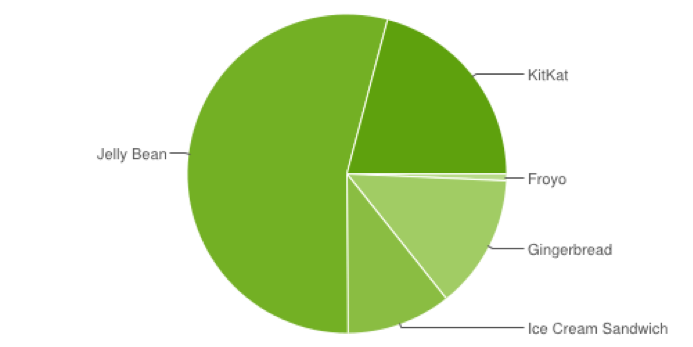
\includegraphics[width=1\textwidth]{Figuras/versionesAndroid.png}
		\rule{30em}{0.5pt}
	\caption[Gráfica de Usabilidad de las Versiones de Android]{Gráfica de Usabilidad de las Versiones de Android (Agosto 2014) \cite{devAndroid}}
	\label{fig:versionesFigura}
\end{figure}

\begin{table} 
	\begin{center}
		\begin{tabular}{|c|c|c|c|}
			\hline \rowcolor[RGB]{51,153,255} 
			\textcolor{blanco}{\bf Versión} &
				\textcolor{blanco}{\bf Nombre} &
				\textcolor{blanco}{\bf API} &
				\textcolor{blanco}{\bf Presencia en el Mercado} \\
			\hline  
				2.2 &
				Froyo &
				8 &
				0.7\% \\
      		\hline \rowcolor[RGB]{240,248,255}
      			2.3.3 - 2.3.7 &
				Gingerbread &
				10 &
				13.6\% \\
      		\hline 
      			4.0.3 - 4.0.4 &
				Ice Cream Sandwich &
				15 &
				10.6\% \\
      		\hline \rowcolor[RGB]{240,248,255}
      			4.1.x &
				Jelly Bean &
				16 &
				26.5\% \\
      		\hline 
      			4.2.x &
				Jelly Bean &
				17 &
				19.8\% \\
      		\hline \rowcolor[RGB]{240,248,255}
      			4.3 &
				Jelly Bean &
				18 &
				7.9\% \\
      		\hline 
      			4.4 &
				KitKat &
				19 &
				20.9\% \\
      		\hline 
		\end{tabular}
	\end{center}
	\caption[Usabilidad de las Versiones de Android]{Usabilidad de las Versiones de Android \cite{devAndroid}} 
	\label{tab:versionesTabla}
\end{table}

\paragraph{Lenguaje de Programación}

La fila correspondiente a lenguajes de programación en la Tabla \ref{tab:comSOM} nos muestra C, C++ y Java como los mas utilizados para Android. En la Tabla \ref{tab:paramLengu} se muestran los parámetros de los lenguajes de programación que aparecen en la Tabla \ref{tab:lenguProgra}, esto con el fin de elegir el lenguaje de programación que se utilizará en este proyecto. 

\begin{table}[h!]
	\begin{center}
		\begin{tabular}{|c|p{4.5cm}|p{4.5cm}|}
			\hline \rowcolor[RGB]{51,153,255} 
			\textcolor{blanco}{\bf Parámetro} &
				\textcolor{blanco}{\bf Descripción} &
				\textcolor{blanco}{\bf Escala de Medición} \\
			\hline 
				Paradigma &
				Enfoque empleado para modelado de un sistema según la naturaleza y filosofía de un lenguaje de programación. &
				Orientado a Objetos, Estructurado, Funcional, Reflexivo, Orientado a eventos. \\
      		\hline \rowcolor[RGB]{240,248,255}
      			Plataformas Compatibles &
				Plataforma donde el lenguaje de programación puede generar código objeto. &
				Android, iOS y Windows Phone. \\
      		\hline 
      			Curva de Aprendizaje &
				Se refiere al tiempo que lleva al equipo de desarrollo dominio y transición. &
				Corta, Media, Larga. \\
      		\hline \rowcolor[RGB]{240,248,255}
      			Complejidad &
				Es la medición relativa sobre la experiencia de trabajo con el paradigma y el lenguaje de programación que lo implementa. &
				Complejo (Sin experiencia), Media (Experiencia en paradigma o sintaxis del lenguaje), Fácil (Experiencia en paradigma y sintaxis del lenguaje). \\
      		\hline 
      			Documentación &
				Muestra la cantidad de información existente. &
				Abundante, Media, Escasa. \\
      		\hline 
    		\end{tabular}
	\end{center}
	\caption[Parámetros de Comparación para el Lenguaje de Programación]{Parámetros de Comparación para el Lenguaje de Programación} 
	\label{tab:paramLengu}
\end{table}

\begin{table} 
	\begin{center}
		\begin{tabular}{|p{3cm}|p{3cm}|p{3cm}|p{3cm}|}
			\hline \rowcolor[RGB]{51,153,255} 
			\textcolor{blanco}{\bf Parámetros} &
				\textcolor{blanco}{\bf C++} &
				\textcolor{blanco}{\bf Java} &
				\textcolor{blanco}{\bf C} \\
			\hline 
				Paradigma &
				Multiparadigma: programación orientada a objetos, programación genérica, programación estructurada, programación funcional y metaprogramación. &
				Multiparadigma: programación orientada a objetos, programación genérica, programación estructurada, programación reflexiva y programación concurrente. & 
				Programación \newline estructurada \\
      		\hline \rowcolor[RGB]{240,248,255}
      			Plataformas Compatibles &
				Multiplataforma &
				Multiplataforma &
				Multiplataforma \\
      		\hline 
      			Curva de \newline Aprendizaje &
				Media &
				Corta &
				Media \\
      		\hline \rowcolor[RGB]{240,248,255}
      			Complejidad &
				Media &
				Fácil &
				Media \\
      		\hline 
      			Documentación &
				Abundante &
				Abundante &
				Abundante \\
      		\hline 
    		\end{tabular}
	\end{center}
	\caption[Comparación de Lenguajes de Programación]{Comparación de Lenguajes de Programación} 
	\label{tab:lenguProgra}
\end{table}
\newpage
En términos de paradigma excluimos al lenguaje C ya que se requiere de programación orientada a objetos. En lo que respecta a la complejidad para el equipo de desarrollor, se muestra que Java es menos complejo que C++, por lo tanto, el lenguaje de programación que se utilizará para TASMC es Java.

\paragraph{Sistema Operativo de Escritorio}

Los sistemas operativos con los que cuenta el equipo de desarrollo se pueden observar en la Tabla \ref{tab:SOE}.

\begin{table}[h] 
	\begin{center}
		\begin{tabular}{|c|c|}
			\hline \rowcolor[RGB]{51,153,255} 
			\textcolor{blanco}{\bf Computadora} &
				\textcolor{blanco}{\bf Sistema Operativo} \\
			\hline 
				Laptop Lenovo &
				Windows 7 \\
      		\hline \rowcolor[RGB]{240,248,255}
      			MacBook Pro &
				OS X Yosemite 10.10.1 \\
      		\hline 
    		\end{tabular}
	\end{center}
	\caption[Sistemas Operativos del Equipo]{Sistemas Operativos del Equipo} 
	\label{tab:SOE}
\end{table}

Debido a que se eligió Android como sistema operativo móvil, visualizando la Tabla \ref{tab:comSOM}, encontramos que las plataformas en donde se puede desarrollar para Android son: Windows, Mac OS y Linux. Por lo tanto, las computadoras que tiene el equipo nos permiten desarrollar TASMC.

\paragraph{Entorno de Desarrollo Integrado}

Un Entorno de desarrollo integrado o IDE como se le conoce comúnmente, es una herramienta de software que permite unificar el control sobre el desarrollo de un sistema, se compone de una gran cantidad de módulos que ayudan a configurar opciones y corregir problemáticas presentes en la sintaxis o lógica del código, permiten el uso de plantillas para agilizar el desarrollo. Debido a la complejidad de los sistemas computacionales actuales, el IDE ha logrado convertirse también en una pieza clave para alcanzar la meta de desarrollo gracias a las ventajas que brinda contra los tiempos de desarrollo.

Dadas las características requeridas por las herramientas establecidas en anterioridad se priorizara que el IDE cumpla con los parámetros de la Tabla \ref{tab:paramIDEs}.

\begin{table}[h]
	\begin{center}
		\begin{tabular}{|p{4.2cm}|p{4.5cm}|p{4.5cm}|}
			\hline \rowcolor[RGB]{51,153,255} 
			\textcolor{blanco}{\bf Parámetros} &
				\textcolor{blanco}{\bf Descripción} &
				\textcolor{blanco}{\bf Escala de Medición} \\
			\hline 
				Soporte para Desarrollo Java (Android) &
				Es preciso que el IDE soporte desarrollo para el lenguaje JAVA y resguarde compatibilidad con el JDK en sus versiones 1.6 y 1.7 además de ser compatible con el ambiente de trabajo para desarrollar aplicaciones Android. &
				Con soporte, sin soporte \\
      		\hline \rowcolor[RGB]{240,248,255}
      			Soporte para Conectividad SQLite &
				Se debe tener una configuración transparente para la comunicación con SQLite, supervisada mediante el IDE. &
				Con soporte, sin soporte. \\
      		\hline 
      			Consumo de Recursos &
				El IDE debe ser congruente con el consumo de recurso, entiéndase como la exigencia de que sea una de las herramientas que consuma menos recursos para el desarrollo. &
				Alta, Media. \\
      		\hline \rowcolor[RGB]{240,248,255}
      			Eficiencia de la configuración  &
				El IDE debe realizar una configuración confiable y fácilmente modificable, para realizar pruebas antes de la puesta a punto. &
				Alta, Media, Baja. \\
      		\hline 
    		\end{tabular}
	\end{center}
	\caption[Parámetros de Comparación para IDEs]{Parámetros de Comparación para IDEs} 
	\label{tab:paramIDEs}
\end{table}

\begin{table}[h]
	\begin{center}
		\begin{tabular}{|p{3cm}|p{3cm}|p{3cm}|}
			\hline \rowcolor[RGB]{51,153,255} 
			\textcolor{blanco}{\bf Parámetros} &
				\textcolor{blanco}{\bf Android Studio} &
				\textcolor{blanco}{\bf Eclipse ADT} \\
			\hline 
				Soporte para Desarrollo Java (Android) &
				Con soporte &
				Con soporte \\
      		\hline \rowcolor[RGB]{240,248,255}
      			Soporte para Conectividad SQLite &
				Con soporte &
				Con soporte \\
      		\hline 
      			Consumo de Recursos &
				Medio &
				Alto \\
      		\hline \rowcolor[RGB]{240,248,255}
      			Eficiencia de la Configuración &
				Alta &
				Media \\
      		\hline 
    		\end{tabular}
	\end{center}
	\caption[Comparacion IDEs Android Studio y Eclipse ADT]{Comparacion IDEs Android Studio y Eclipse ADT} 
	\label{tab:comIDEs}
\end{table}

Como se puede observar Android Studio y Eclipse ADT son IDEs muy semejantes, la principal diferencia entre ambos es que Android Studio esta recibiendo más soporte que el mismo Eclipse ADT hoy en día. Debido a que Android Studio consume menos recursos y, además, el sistema de construcción que utiliza es Gradle, se utilizará éste IDE para el desarrollo de TASMC.

\paragraph{Herramienta UML}

StartUML es una de las herramientas open source para un desarrollo rápido, flexible, extensible basado en los estándares UML (Unified Modeling Lenguage) y MDA (Model Driven Arquitecture), esta herramienta corre sobre sistemas operativos Windows y Mac OS. StarUML ofrece un amplio grupo de diagramas de UML 2.0, entre los cuales están: Diagramas de casos de uso, diagrama de clases, diagrama de secuencia, diagrama de comunicación, diagrama de máquina de estado, diagrama de actividad, diagrama de componentes, diagrama de despliegue, diagrama de estructura compuesta (UML 2.0). Al igual que soporta varios lenguajes entre los cuales se encuentra Java, C++, C\# (generador de código y de ingeniería inversa). \cite{starUML}

Debido a que StarUML es gratuita, se apega a los estándares UML y se puede utilizar tanto en Windows como Mac OS, utilizaremos StarUML como herramienta UML para nuestro proyecto.
\newpage
\paragraph{Sistema Gestor de Base de Datos}

\begin{table}[h!]
	\begin{center}
		\begin{tabular}{|p{3cm}|p{5.1cm}|p{5.1cm}|}
			\hline \rowcolor[RGB]{51,153,255} 
			\textcolor{blanco}{\bf Parámetro} &
				\textcolor{blanco}{\bf SQLite} &
				\textcolor{blanco}{\bf Oracle Lite} \\
			\hline 
				Paradigma &
				Relacional &
				Relacional \\
      		\hline \rowcolor[RGB]{240,248,255}
      			Costo de Licencia &
				SQLite es de dominio público, y por tanto, no tiene costo y se puede redistribuir libremente. &
				\$ 180 USD por licencia \\
      		\hline 
      			Interfaces &
				Cuenta con diferentes interfaces del API para trabajar con C++, PHP, Perl, Python, etc. &
				Interfaz GUI y SQL. \\
      		\hline \rowcolor[RGB]{240,248,255}
      			Tamaño &
				SQLite tiene una pequeña memoria y una única biblioteca es necesaria para acceder a bases de datos, esto lo hace ideal para aplicaciones de bases de datos incorporadas. El tamaño máximo de una base de datos es de 2 TB. &
				 La carga sobre el dispositivo móvil es mínima ya que los datos y aplicaciones se almacenan en servidores móviles los cuales a su vez se comunican con un repositorio propio de Oracle. \\
      		\hline 
      		Portabilidad &
      		Se ejecuta en muchas plataformas y sus bases de datos pueden ser fácilmente portadas sin ninguna configuración o administración. &
      		Se ejecuta en múltiples plataformas, incluyendo Android, iPhone (Apple iOS), Blackberry, Symbian OS, Windows de 32 bits, Windows Mobile, Linux y otras plataformas de dispositivos móviles. \\
      		\hline \rowcolor[RGB]{240,248,255}
      		Rendimiento &
      		SQLite realiza operaciones de manera eficiente y es más rápido que MySQL y PostgreSQL. &
      		Ofrece un rendimiento fuera de la caja, permitiendo a los usuarios el acceso información de forma rápida y eficiente. Multiprocesador y la memoria caché dinámica dimensionamiento garantizar arriba rendimiento para las bases de datos más grandes y un mayor número de usuarios conectados. \\ 
      		\hline 
      		Estabilidad &
      		SQLite es compatible con ACID, reunión de los cuatro criterios de Atomicidad, Consistencia, Aislamiento y Durabilidad. &
      		Oracle es compatible con ACID, además de manejar integridad referencial, transacciones y  estándar de codificación Unicode. \\
      		\hline
    		\end{tabular}
	\end{center}
	\caption[Comparación SGBD móviles]{Comparación SGBD móviles} 
	\label{tab:comSGBD}
\end{table}
\newpage
El gestor de base de datos es el software que se ocupa del almacenamiento, modificación y extracción de la información procedente de una base de datos. Representa una interfaz de comunicación entre la entrada de información y los registros almacenados en repositorios. Además forma parte medular para la implementación de todo sistema que almacena información en bases de datos. En la Tabla \ref{tab:comSGBD} se encuentran los SGBD, para móviles, que se pueden utilizar para el desarrollo de TASMC.

En términos de consumo de recursos, rendimiento y costo se eligió utilizar SQLite como gestor de base de datos, dado que para la implementación del sistema se pensó en utilizar un SGBD capaz de reaccionar ágilmente ante la concurrencia de solicitudes al tiempo que consume bajos recursos, además de que no es necesario una base de datos tan robusta.

\paragraph{API de Rutas de Google Maps}

El API de rutas de Google es un servicio que utiliza una solicitud HTTP para calcular rutas para llegar de una ubicación a otra. Puedes buscar rutas de varios métodos de transporte, como en transporte público, en coche, a pie o en bicicleta. Las rutas pueden especificar los orígenes, los destinos y los hitos como cadenas de texto (por ejemplo, ``Chicago, IL'' o ``Darwin, NT, Australia'') o como coordenadas de latitud/longitud. El API de rutas puede devolver rutas segmentadas mediante una serie de hitos.

Por lo general, este servicio está diseñado para calcular rutas a partir de direcciones estáticas (conocidas previamente) para la ubicación del contenido de la aplicación en un mapa. Sin embargo, este servicio no está diseñado para responder en tiempo real a la información introducida por el usuario.

El cálculo de indicaciones es un proceso que consume mucho tiempo y muchos recursos. Siempre que sea posible, se debe realiza un cálculo previo de las direcciones conocidas (mediante el servicio descrito) y almacena los resultados en una memoria caché. \cite{apiGoogleMaps}
\newpage
\paragraph{API de IndoorAtlas}

El API de Indooratlas nos ayudará a realizar la localización en interiores sin necesidad de utilizar infraestructura de hardware externo. \cite{apiIndoorAtlas}

Lo que Indooratlas nos ofrece:

\begin{itemize}
	\item 2 metros de precisión en la localización.
	\item	Ahorro de recursos si lo comparamos con otra técnica para la localización en interiores.
	\item Una solución multiplataforma para iOS y Android.
\end{itemize}

\subsection{Factibilidad Ecónomica}

El estudio de factibilidad económica permite analizar los costos y beneficios económicos que se obtendrán con el desarrollo del proyecto, sin importar que la implementación de nuestro sistema sea un prototipo sin fines lucrativos. 
\vspace{2cm}
\begin{table}[h]
	\begin{center}
		\begin{tabular}{|c|c|c|c|c|}
			\hline \rowcolor[RGB]{51,153,255} 
			\textcolor{blanco}{\bf Recurso} &
				\textcolor{blanco}{\bf Cantidad} &
				\textcolor{blanco}{\bf Meses} &
				\textcolor{blanco}{\bf Salario Mensual} &
				\textcolor{blanco}{\bf Total} \\
			\hline 
				Líder de proyecto &
				1 &
				8 &
				\$ 35,000.00 &
				\$ 280,000.00 \\
      		\hline \rowcolor[RGB]{240,248,255}
      			Desarrollador &
				2 &
				8 &
				\$ 23,000.00 &
				\$ 368,000.00 \\
      		\hline 
    		\end{tabular}
	\end{center}
	\caption[Recursos Humanos]{Recursos Humanos \cite{salarios}} 
	\label{tab:recursosHumanos}
\end{table}

\begin{table}[h]
	\begin{center}
		\begin{tabular}{|c|c|c|c|}
			\hline \rowcolor[RGB]{51,153,255} 
			\textcolor{blanco}{\bf Recurso} &
				\textcolor{blanco}{\bf Cantidad} &
				\textcolor{blanco}{\bf Precio Unitario} &
				\textcolor{blanco}{\bf Total} \\
			\hline
				Impresiones y fotocopias &
				5,000 &
				\$ 0.50 &
				\$ 2,500.00  \\
      		\hline \rowcolor[RGB]{240,248,255}
      			Gastos varios &
				&
				&
				\$ 500.00 \\
      		\hline 
    		\end{tabular}
	\end{center}
	\caption[Recursos Consumibles]{Recursos Consumibles} 
	\label{tab:recursosConsumibles}
\end{table}

\begin{table}[h] 
	\begin{center}
		\begin{tabular}{|c|c|c|c|}
			\hline \rowcolor[RGB]{51,153,255} 
			\textcolor{blanco}{\bf Recurso} &
				\textcolor{blanco}{\bf Cantidad} &
				\textcolor{blanco}{\bf Costo} &
				\textcolor{blanco}{\bf Total} \\
			\hline 
				Laptop Lenovo &
				1 &
				\$ 9,000.00 &
				\$ 9,000.00  \\
      		\hline \rowcolor[RGB]{240,248,255}
      			MacBook Pro &
				1 &
				\$ 19,000.00&
				\$ 19,000.00 \\
			\hline 
				Samsung Galaxy S4 &
				1 &
				\$ 7,000.00 &
				\$ 7,000.00  \\
      		\hline \rowcolor[RGB]{240,248,255}
      			Google Maps Services &
				1 &
				\$ 0 &
				\$ 0 \\
			\hline
				IndoorAtlas Services &
				1 &
				\$ 0 &
				\$ 0 \\
      		\hline \rowcolor[RGB]{240,248,255}
      			Web Service Vuelos &
				1 &
				\$ 0 &
				\$ 0 \\
			\hline
				Servidor TASMC &
				1 &
				\$ 4,000.00 &
				\$ 4,000.00 \\	
      		\hline 
    		\end{tabular}
	\end{center}
	\caption[Recursos Tecnológicos]{Recursos Tecnológicos} 
	\label{tab:recursosTecnologicos}
\end{table}

\begin{table} 
	\begin{center}
		\begin{tabular}{|c|c|}
			\hline \rowcolor[RGB]{51,153,255} 
			\textcolor{blanco}{\bf Recurso} &
				\textcolor{blanco}{\bf Total} \\
			\hline 
				Recursos Humano &
				\$ 648,000.00  \\
      		\hline \rowcolor[RGB]{240,248,255}
      			Recursos Consumibles &
				\$ 3,000.00  \\
			\hline 
				Recursos Tecnológicos &
				\$ 39,000.00  \\
      		\hline \rowcolor[RGB]{240,248,255}
      			Subtotal &
				\$ 690,000.00  \\
			\hline  
				Imprevistos (10 \%) &
				\$ 70,000.00  \\
      		\hline \rowcolor[RGB]{240,248,255}
      			Total &
				\$ 760,000.00 \\
      		\hline 
    		\end{tabular}
	\end{center}
	\caption[Costo Total TASMC]{Costo Total TASMC} 
	\label{tab:costoTasmc}
\end{table}
\vspace{3cm}
\newpage
\subsection{Factibilidad Operativa}

El estudio de factibilidad operativa nos ayuda a determinar si el proyecto puede ser implementado y completado para lograr sus objetivos. Puede ser visto desde dos puntos: recursos humanos para la implementación del proyecto y recursos necesarios para la puesta en marcha del proyecto. 

\textbf{Recursos humanos para la implementación del proyecto}

El equipo de trabajo cuenta con los conocimientos necesarios para el desarrollo del proyecto, mediante las tecnologías seleccionadas. Por lo que es factible que el proyecto sea implementado. 

\textbf{Recursos necesarios para la puesta en marcha del proyecto}

El proyecto se quedará como un prototipo, por lo que no se necesitan recursos extras para una implantación y puesta en marcha del sistema dentro de una empresa, aunque el proyecto puede ser extendido o mejorado para su implantación.

En la Tabla \ref{tab:fodaTASMC} se muestra el FODA de TASMC:

\begin{table}[h]
	\begin{center}
		\begin{tabular}{|p{6.8cm}|p{6.8cm}|}
			\hline  
				\textbf{\small Fortalezas:} & \textbf{\small Debilidades:} \\
				{\parbox{0.45\textwidth}{
					\begin{itemize}
                			\item \small Ser un sistema único de gestión integral de viajes.
						\item \small Creación de un sistema totalmente personalizado y a la medida.
						\item \small Preocupación y esmero por el buen diseño estético y  funcional de la aplicación.
           			\end{itemize} }} &
				{\parbox{0.45\textwidth}{
					\begin{itemize}
                			\item \small Poca publicidad de la aplicación.
						\item \small No contar con los planos del AICM.
						\item \small Menor disponibilidad de recursos. 
           			\end{itemize} }}	\\
			\hline 
			\textbf{\small Oportunidades:} & \textbf{\small Amenazas:} \\
				{\parbox{0.45\textwidth}{
					\begin{itemize}
                			\item \small Ampliación de mercado en el desarrollo de aplicaciones móviles.
						\item \small Alta intensidad en el uso de aplicaciones móviles.
           			\end{itemize} }} &
				{\parbox{0.45\textwidth}{
					\begin{itemize}
                			\item \small Compañías transnacionales que se dedican al desarrollo de aplicaciones móviles. 
						\item \small Posible existencia de aplicaciones similares que cuenten con mejor infraestructura de operación. 
           			\end{itemize} }}	\\
			\hline 
		\end{tabular}
	\end{center}
	\caption[FODA TASMC]{FODA TASMC} 
	\label{tab:fodaTASMC}
\end{table}
\section{Análisis de Requerimientos}

Dentro de esta etapa, a partir de las reglas de negocio y la descripción del sistema se debe considerar la obtención de los requerimientos básicos, los cuales cumplen la función de definir de manera general el sistema a desarrollar para después pasar a especificar los requerimientos funcionales que nos reflejen a detalle las funciones que el sistema debe o no efectuar.

Los requerimientos no funcionales son restricciones a las funciones del sistema o bien cualidades que este debe de presentar para considerarle un sistema de calidad.

\subsection{Reglas de Negocio}

Las reglas de negocio especifican procesos, operaciones, normas y restricciones consideradas en el desarrollo de software dependiendo de la metodología que se emplea para resolver el problema y lograr los objetivos. Las reglas del negocio son usadas para verificar que ciertos comportamientos se cumplan y en caso de que se presente una excepción conocer las alternativas para la solución del problema.

\begin{table}
	\begin{center}
		\begin{tabular}{|c|c|p{3cm}|p{5.7cm}|}
			\hline \rowcolor[RGB]{0,102,204} 
				\textcolor{blanco}{\bf Identificador} &
				\textcolor{blanco}{\bf Tipo} &
				\textcolor{blanco}{\bf Nombre} &
				\textcolor{blanco}{\bf Descripción} \\
			\hline \rowcolor[RGB]{224,224,224} 
				\textbf{RN01} &
				Definición &
				Viajero aéreo &
				Persona que viaja en un avión. \\
      		\hline 
      			\textbf{RN02} &
				Definición &
				Viaje aéreo &
				Traslado de un lugar a otro, mediante la  utilizando aeronaves, con fin lucrativo. \\
			\hline \rowcolor[RGB]{224,224,224} 
				\textbf{RN03} &
				Definición &
				Aerolínea &
				Empresa o compañía dedicada al transporte aéreo. \\ 
			\hline
				\textbf{RN04} &
				Definición &
				Vuelo &
				Trayecto que realiza un avión, haciendo o no escalas, entre el punto de origen y el destino. \\ 
			\hline \rowcolor[RGB]{224,224,224} 
				\textbf{RN05} &
				Hecho &
				Visualizar los vuelos de las aerolíneas. &
				El viajero aéreo puede ver todos los vuelos que las aerolíneas proporcionan, sin importar que falten semanas o meses para el vuelo. \\ 
			\hline
				\textbf{RN06} &
				Definición &
				Itinerario de viaje &
				Listado en el que se describen los lugares por los que se va a pasar. \\ 
			\hline \rowcolor[RGB]{224,224,224} 
				\textbf{RN07} &
				Hecho &
				Notificar al viajero &
				El viajero debe ser notificado en caso de producirse algún cambio en cuanto al vuelo o el horario. \\ 
			\hline
				\textbf{RN08} &
				Hecho &
				Recordar documentos importantes &
				Se debe apoyar al viajero en que no olvide documentos importantes para su viaje. \\ 
			\hline \rowcolor[RGB]{224,224,224} 
				\textbf{RN09} &
				Hecho &
				Puntualidad en el aeropuerto &
				El viajero debe llegar puntual a la cita en el aeropuerto para cumplir con los procedimientos que necesita para el abordaje del avión. \\ 
			\hline
				\textbf{RN10} &
				Hecho &
				Guardar objetos importantes &
				El viajero no debe olvidar objetos importantes para contribuir con la satisfacción total del viaje. \\ 
			\hline \rowcolor[RGB]{224,224,224} 
				\textbf{RN11} &
				Hecho &
				Hoteles en la ciudad destino &
				Se debe informar al viajero sobre los hoteles que se encuentren en la ciudad destino.  \\ 
			\hline
				\textbf{RN12} &
				Hecho &
				Usabilidad &
				Se debe asistir al viajero, para que pueda cumplir con un viaje satisfactorio, apoyándolo con la gestión de su viaje de una manera sencilla y comprensible.  \\ 
			\hline \rowcolor[RGB]{224,224,224} 
				\textbf{RN13} &
				Hecho &
				Disponibilidad &
				La información debe estar disponible idealmente todo el año.  \\ 
			\hline
				\textbf{RN14} &
				Hecho &
				Información del AICM &
				El viajero debe conocer el teléfono, dirección, mapa, etc. del aeropuerto para cualquier situación o necesidad que se presente. \\ 
			\hline 
		\end{tabular}
	\end{center}
	\caption[Reglas de Negocio]{Reglas de Negocio} 
	\label{tab:reglasNegocio}
\end{table}

\subsection{Requerimientos Básicos (RB)}

Las características que contendrá TASMC son las siguientes:

\begin{itemize}
	\item Guardar configuración personal de cada usuario al registrarse
	\item Búsqueda de Hoteles
	\item Lista de Hoteles
	\item Búsqueda de Vuelos
	\item Lista de Vuelos
	\item Lista de información del AICM
	\item Lista de Objetos para viaje
	\item Itinerario de viaje
	\item Ruta casa-aeropuerto
	\item Ubicación dentro del Aeropuerto
\end{itemize}

En base a las características que debe contener TASMC se han podido identificar los diferentes módulos de la aplicación que se encuentran listados a continuación:

\textbf{Módulo de Registro/Configuración}

\begin{itemize}
	\item Correo electrónico.
	\item Clase de vuelo preferida.
	\item Cantidad preferida de estrellas en hotel. 
\end{itemize}

\textbf{Módulo de Hoteles}

\begin{itemize}
	\item Búsqueda de Hoteles.
	\begin{itemize}
		\item Número de Huéspedes.
		\item Número de Habitaciones.
		\item Fecha de entrada y salida.
	\end{itemize}
	\item Listado de Hoteles.
	\item Detalle de Hoteles.
	\item Filtros según:
	\begin{itemize}
		\item Estrellas: de 1 a 5.
		\item Estrellas: de 5 a 1.
		\item Precios de bajo a alto.
		\item Precios de alto a bajo.
	\end{itemize}
\end{itemize}

\textbf{Modulo de Vuelos}
 
\begin{itemize}
	\item Búsqueda de Vuelos
	\begin{itemize}
		 \item Número de pasajeros.
		\item Clase (Económico, Económico Premium, Business, Primera, Todas).
		\item Fechas (Salida y llegada).
		\item Ciudad origen – Ciudad destino.
	\end{itemize}
	\item Listado de Vuelos.
	\item Detalle de Vuelos.
	\item Filtros según:
	\begin{itemize}
		\item Precios de bajo a alto.
		\item Precios de alto a bajo.
		\item Clase de vuelo.
	\end{itemize}
\end{itemize}

\textbf{Información Aeropuerto AICM}

\begin{itemize}
	\item Información de Aeropuerto AICM
	\begin{itemize}
		 \item Sitio web AICM.
		\item Teléfono AICM.
		\item Ubicación.
	\end{itemize}
	\item Mapa del Aeropuerto.
	\item	Servicios en el Aeropuerto.
\end{itemize}

\textbf{Lista de equipaje}

\begin{itemize}
	\item 	Lista de equipaje por tipo de vuelo.
	\item Lista de equipaje.
	\item Añadir nueva lista.
	\item Añadir nuevo objeto.
	\item Documentos importantes
\end{itemize}
	
\textbf{Itinerario}

\begin{itemize}
	\item Alarma según tipo de vuelo:
	\begin{itemize}
		\item Nacional 3.5 Horas antes de hora de salida.
		\item Internacional 4.5 Horas antes de hora de salida.
	\end{itemize}
	\item Información de vuelo
	\begin{itemize}
		\item Número de vuelo.
		\item Hora de salida.
		\item Hora de llegada.
	\end{itemize}
	\item Itinerario de viaje
	\begin{itemize}
	 \item Actividades a realizar durante el viaje.
	\end{itemize}
\end{itemize}

\textbf{Ruta para llegar al AICM}

\begin{itemize}
	\item Visualizar una ruta para llegar al AICM.
\end{itemize}

\textbf{Ubícate}

\begin{itemize}
	\item Ubicar sala de abordaje del usuario.
	\item Ubicar servicios del AICM.
\end{itemize} 

\textbf{Información de Vuelo}

\begin{itemize}
	\item Número de vuelo.
	\item Estado de vuelo.
	\item Ciudad de origen.
	\item Ciudad destino.
	\item Hora de salida.
	\item Hora de llegada.
	\item Fecha.
	\item Terminal.
	\item Puerta.
\end{itemize}

\begin{table}
	\begin{center}
		\begin{tabular}{|c|p{8.4cm}|p{2.5cm}|}
			\hline \rowcolor[RGB]{0,102,204} 
				\textcolor{blanco}{\bf Identificador} &
				\textcolor{blanco}{\bf Descripción} &
				\textcolor{blanco}{\bf Origen} \\
			\hline \rowcolor[RGB]{224,224,224} 
				\textbf{RB01} &
				Módulo que permita al usuario realizar su registro a TASMC y elegir sus preferencias. &
				Definición del sistema  \\
      		\hline 
      			\textbf{RB02} &
				Módulo para realizar búsquedas de Hoteles y posteriormente generar un listado de dicha búsqueda. &
				Definición del sistema, RN11 \\
			\hline \rowcolor[RGB]{224,224,224} 
				\textbf{RB03} &
				Módulo para realizar búsquedas de Vuelos y posteriormente generar un listado de dicha búsqueda. &
				Definición del sistema, RN05 \\ 
			\hline
				\textbf{RB04} &
				Módulo para visualizar la información del AICM, como sitio web, teléfono, ubicación y redes sociales. &
				Definición del sistema, RN14 \\ 
			\hline \rowcolor[RGB]{224,224,224} 
				\textbf{RB05} &
				Módulo para la gestión de objetos, donde el usuario podrá verificar en una lista los objetos requeridos para su viaje. &
				Definición del sistema, RN10 \\ 
			\hline
				\textbf{RB06} &
				Módulo para asistir en la construcción del itinerario de viaje del usuario. &
				Definición del sistema \\ 
			\hline \rowcolor[RGB]{224,224,224} 
				\textbf{RB07} &
				Módulo que permita visualizar rutas que tengan como destino el AICM. &
				Definición del sistema, RN09, RN12 \\ 
			\hline
				\textbf{RB08} &
				Módulo que permita visualizar en un mapa del AICM la ubicación del usuario en el momento que lo requiera. &
				Definición del sistema, RN12 \\ 
			\hline \rowcolor[RGB]{224,224,224} 
				\textbf{RB09} &
				Módulo para visualizar la información del vuelo, como lo es, el número de vuelo, el estado de vuelo, ciudad de origen, ciudad destino, hora de salida, hora de llegada, fecha, terminal y puerta. &
				Definición del sistema, RN07 \\ 
			\hline 
		\end{tabular}
	\end{center}
	\caption[Requerimientos Básicos]{Requerimientos Básicos} 
	\label{tab:reqBasicos}
\end{table}

\subsection{Requerimientos Funcionales (RF)}

En la siguiente tabla se muestran los requerimientos funcionales de TASMC:

\begin{table}
	\begin{center}
		\begin{tabular}{|c|p{9.4cm}|p{1.5cm}|}
			\hline \rowcolor[RGB]{0,102,204} 
				\textcolor{blanco}{\bf Identificador} &
				\textcolor{blanco}{\bf Descripción} &
				\textcolor{blanco}{\bf Origen} \\
			\hline \rowcolor[RGB]{224,224,224} 
				\textbf{RF01} &
				El sistema debe ser capaz de configurar gustos y posibilidades económicas del viajero para generar un mejor resultado en la búsqueda de vuelos y hoteles. &
				RB01 \\
      		\hline 
      			\textbf{RF02} &
				El usuario debe poder visualizar sugerencias de hoteles disponibles,  según una búsqueda que haya realizado previamente. &
				RB02 \\
			\hline \rowcolor[RGB]{224,224,224} 
				\textbf{RF03} &
				El usuario debe poder visualizar sugerencias de vuelos disponibles, según una búsqueda que haya realizado previamente. &
				RB03 \\ 
			\hline
				\textbf{RF04} &
				El sistema debe ser capaz de generar una lista de objetos que debe empacar el usuario, según el tipo de viaje que se seleccione. &
				RB05 \\ 
			\hline \rowcolor[RGB]{224,224,224} 
				\textbf{RF05} &
				El sistema debe proporcionar una lista que permita al usuario generar un itinerario de viaje. &
				RB06 \\ 
			\hline
				\textbf{RF06} &
				El sistema mostrará una sugerencia de la mejor ruta para llegar al AICM desde la posición actual del usuario. &
				RB07 \\ 
			\hline \rowcolor[RGB]{224,224,224} 
				\textbf{RF07} &
				El sistema debe ser capaz de ubicar al usuario dentro del AICM y facilitarle la llegada a su sala de abordaje. &
				RB08 \\ 
			\hline
				\textbf{RF08} &
				El sistema deberá mostrar la información del número de vuelo, estado de vuelo, ciudades de origen y destino, 					hora de salida y llegada, fecha, terminal y puerta. &
				RB09 \\ 
			\hline
		\end{tabular}
	\end{center}
	\caption[Requerimientos Funcionales]{Requerimientos Funcionales} 
	\label{tab:reqFuncionales}
\end{table}

\subsection{Requerimientos No Funcionales (RNF)}

En la siguiente tabla se muestran los requerimientos no funcionales de TASMC:

\begin{table}
	\begin{center}
		\begin{tabular}{|c|p{8.4cm}|p{2.5cm}|}
			\hline \rowcolor[RGB]{0,102,204} 
				\textcolor{blanco}{\bf Identificador} &
				\textcolor{blanco}{\bf Descripción} &
				\textcolor{blanco}{\bf Origen} \\
			\hline \rowcolor[RGB]{224,224,224} 
				\textbf{RNF01} &
				Las condiciones del entorno no deben de afectar la localización del usuario. Se debe de considerar un ambiente controlado. &
				RB08 \\
      		\hline 
      			\textbf{RNF02} &
				La aplicación debe funcionar en todos los dispositivos móviles que contengan el sistema operativo Android versión 4.4 (KitKat). &
				Definición del Sistema \\
			\hline \rowcolor[RGB]{224,224,224} 
				\textbf{RNF03} &
				Se debe de presentar una interfaz gráfica para poder seleccionar las distintas funciones que puede utilizar el usuario en el sistema. &
				RN12 \\ 
			\hline
				\textbf{RNF04} &
				El sistema debe enviar una respuesta con una rapidez acorde al ancho de banda y la disponibilidad de la red. &
				Definición del Sistema \\ 
			\hline \rowcolor[RGB]{224,224,224} 
				\textbf{RNF05} &
				El sistema debe tener la posibilidad de generar ampliaciones de funcionalidad y escalabilidad. &
				Definición del Sistema \\ 
			\hline
				\textbf{RNF06} &
				Se debe dar soporte continuo al sistema. &
				RN12 \\ 
			\hline \rowcolor[RGB]{224,224,224} 
				\textbf{RNF07} &
				La navegación del usuario dentro de la aplicación debe ser de fácil entendimiento y de manera intuitiva. &
				RB12 \\ 
			\hline
		\end{tabular}
	\end{center}
	\caption[Requerimientos No Funcionales]{Requerimientos No Funcionales} 
	\label{tab:reqNoFuncionales}
\end{table}
\section{Análisis de Riesgos}

El proceso de análisis de riesgos es de utilidad para conocer y de alguna manera tratar de reducir algunas actividades, ideas o actitudes que amenazan con la completa y eficaz elaboración del proyecto.

El primer paso para llevar a cabo el análisis de riesgos es identificarlos. Una manera sencilla para identificar los riesgos es incluirlos dentro de alguna de las siguientes clasificaciones: riesgos organizacionales, riesgos sobre el personal, riesgos tecnológicos, riesgos sobre cambios en los requerimientos y riesgos sobre las herramientas.

Una vez identificados y clasificados los riesgos se hace una valoración de la probabilidad de ocurrencia que tiene cada uno mediante una clasificación por rangos de probabilidad como la Tabla \ref{tab:probabilidadRiesgos}.

\begin{table}[h]
	\begin{center}
		\begin{tabular}{|c|c|}
			\hline \rowcolor[RGB]{51,153,255} 
				\textcolor{blanco}{\bf Probabilidad en \%} &
				\textcolor{blanco}{\bf Valoración} \\
			\hline 
				0\% - 10\% &
				Muy bajo \\
      		\hline \rowcolor[RGB]{240,248,255}
				10\% - 25\% &
				Bajo \\
			\hline 
				25\% - 50\% &
				Moderado \\ 
			\hline \rowcolor[RGB]{240,248,255}
				50\% - 75\% &
				Alto \\ 
			\hline
				75\% - 100\% &
				Muy Alto \\ 
			\hline
		\end{tabular}
	\end{center}
	\caption[Clasificación de Riesgos Conforme a su Probabilidad]{Clasificación de Riesgos Conforme a su Probabilidad} 
	\label{tab:probabilidadRiesgos}
\end{table}

Una vez que cada riesgo tiene asignada una valoración se procede a determinar el efecto que el riesgo tendrá en caso de que se llegara a cumplir. Una manera sencilla para determinar el efecto de cada riesgo es asignar una de las siguientes clasificaciones: catastrófico, serio, tolerable e insignificante. Cada una de las clasificaciones anteriores está ordenada en forma descendente conforme a la valoración de su impacto.

Cuando se han seguido todos los pasos para el proceso de análisis de riesgos el resultado es una tabla donde se muestra el nombre del riesgo, su clasificación, su valoración y su impacto. Los riesgos presentados en la Tabla \ref{tab:analisisRiesgos} deben ser ordenados de manera descendente conforme a su impacto.

\begin{table}[h]
	\begin{center}
		\begin{tabular}{|>{\columncolor[RGB]{51,153,255}}p{6.6cm}|c|c|c|}
			\hline \rowcolor[RGB]{51,153,255} 
				\textcolor{blanco}{\bf Riesgo} &
				\textcolor{blanco}{\bf Clasificación} &
				\textcolor{blanco}{\bf Valoración} &
				\textcolor{blanco}{\bf Efecto} \\		
			\hline
				\textcolor{blanco}{\bf Mala comunicación entre los integrantes del equipo} &
				Organizacional &
				Alto &
				Serio \\
			\hline
				\textcolor{blanco}{\bf Recursos insuficientes para concluir el proyecto} &
				\cellcolor[RGB]{240,248,255}  Organizacional &
				\cellcolor[RGB]{240,248,255}Alto &
				\cellcolor[RGB]{240,248,255}Serio \\
      		\hline 
				\textcolor{blanco}{\bf Retraso de las actividades del proyecto} &
				Organizacional &
				Bajo &
				Serio \\
			\hline  
				\textcolor{blanco}{\bf Falta de responsabilidad de los integrantes del equipo} &
				\cellcolor[RGB]{240,248,255}Personal &
				\cellcolor[RGB]{240,248,255}Bajo &
				\cellcolor[RGB]{240,248,255}Serio \\
			\hline
				\textcolor{blanco}{\bf Mala distribución de actividades} &
				Organizacional &
				Bajo &
				Serio \\
			\hline 
				\textcolor{blanco}{\bf Permiso denegado para realizar trabajos dentro del AICM} &
				\cellcolor[RGB]{240,248,255}Tecnológico &
				\cellcolor[RGB]{240,248,255}Moderado &
				\cellcolor[RGB]{240,248,255}Serio \\
			\hline
				\textcolor{blanco}{\bf Mal control de las versiones del proyecto.} &
				Organizacional &
				Moderado &
				Serio \\
			\hline 
				\textcolor{blanco}{\bf Baja definitiva de alguno de los integrantes del equipo.} &
				\cellcolor[RGB]{240,248,255}Personal &
				\cellcolor[RGB]{240,248,255}Muy Bajo &
				\cellcolor[RGB]{240,248,255}Serio \\
			\hline
				\textcolor{blanco}{\bf Cambios en los requerimientos del sistema por parte de los sinodales} &
				Requerimientos &
				Alto &
				Serio \\
			\hline 
				\textcolor{blanco}{\bf Enfermedad de alguno de los miembros del equipo.} &
				\cellcolor[RGB]{240,248,255}Personal &
				\cellcolor[RGB]{240,248,255}Bajo &
				\cellcolor[RGB]{240,248,255}Tolerable \\
			\hline
				\textcolor{blanco}{\bf Rendimiento no competitivo del sistema} &
				Tecnológico &
				Alto &
				Serio \\
			\hline 
				\textcolor{blanco}{\bf Ausencia de algún integrante del equipo por un periodo prolongado de tiempo} &
				\cellcolor[RGB]{240,248,255}Personal &
				\cellcolor[RGB]{240,248,255}Muy Alto &
				\cellcolor[RGB]{240,248,255}Tolerable \\
			\hline
				\textcolor{blanco}{\bf Falta de dominio de las herramientas de desarrollo} &
				Personal &
				Moderado &
				Tolerable \\
			\hline 
				\textcolor{blanco}{\bf Falla en los dispositivos móviles de prueba} &
				\cellcolor[RGB]{240,248,255}Tecnológico &
				\cellcolor[RGB]{240,248,255}Alto &
				\cellcolor[RGB]{240,248,255}Tolerable \\
			\hline
				\textcolor{blanco}{\bf Funcionamiento inadecuado en la implementación de alguna tecnología después de haber sido calificada como adecuada en el Estudio de Factibilidad} &
				Tecnológico &
				Alto &
				Serio \\
			\hline 
				\textcolor{blanco}{\bf Incorrecta definición de la problemática del proyecto} &
				\cellcolor[RGB]{240,248,255}Organizacional &
				\cellcolor[RGB]{240,248,255}Muy Alto &
				\cellcolor[RGB]{240,248,255}Serio \\
			\hline
		\end{tabular}
	\end{center}
	\caption[Análisis de Riesgos]{Análisis de Riesgos} 
	\label{tab:analisisRiesgos}
\end{table}

\textbf{Identificación de Riesgos}
\newline
Los riesgos han sido identificados clasificados, según el foco de interés, de la siguiente manera:

\begin{itemize}
	\item Ambiente del proyecto
	\item Inventario de activos e intangibles
	\item Mantenimiento de software y hardware
	\item Equipo de trabajo 
	\item Errores de estimación de costos 
\end{itemize}
\clearpage
\textbf{Estrategias para la mitigación de riesgos}
\newline

\begin{table}[h]
	\begin{center}
		\begin{tabular}{|p{14.2cm}|}
			\hline \rowcolor[RGB]{51,153,255} 
				\textcolor{blanco}{\bf Estrategia de mitigación} \\ 
			\hline 
				Seguimiento semanal de los hitos definidos por cada actividad en el desarrollo del proyecto. \\
      		\hline \rowcolor[RGB]{240,248,255} 
				Continúa capacitación del personal durante las horas de trabajo. \\
			\hline 
				Designación de considerable tiempo para esta actividad. \\ 
			\hline \rowcolor[RGB]{240,248,255}
				Conocimiento y seguimiento de la situación laboral y personal de cada miembro del equipo. \\ 
			\hline 
				Realización de pruebas como actividades de capacitación de las tecnologías a usar antes de ser implementadas. \\ 
			\hline \rowcolor[RGB]{240,248,255}
				Realización de pruebas al sistema para poder evitar el mal funcionamiento de alguno de los módulos \\ 
			\hline
				Planificación de todas las actividades antes de comenzar con el proyecto y fijar una fecha de entrega anterior a la acordada con el cliente pues esto nos dará una holgura de tiempo \\ 
			\hline \rowcolor[RGB]{240,248,255}
				Buscar y utilizar herramientas que se adapten a todos los dispositivos \\ 
			\hline
				Mantener una actitud positiva para manejar  los problemas y regirse conforme a la planeación \\ 
			\hline
		\end{tabular}
	\end{center}
	\caption[Plan de Mitigación]{Plan de Mitigación} 
	\label{tab:planMitigacion}
\end{table}

\textbf{Planes de contingencia}
\newline

\begin{table}[h]
	\begin{center}
		\begin{tabular}{|p{14.2cm}|}
			\hline \rowcolor[RGB]{51,153,255} 
				\textcolor{blanco}{\bf Planes de contingencia} \\
			\hline 
				Compensar el tiempo de retraso con horas de trabajo extra. \\
      		\hline \rowcolor[RGB]{240,248,255}
				Capacitación personal para el personal incompetente en horas extra de trabajo. \\
			\hline 
				Dialogo en el  equipo de trabajo si existe una mala definición en la problemática del proyecto para hacer un replanteamiento de la problemática. \\ 
			\hline \rowcolor[RGB]{240,248,255}
				Distribución del trabajo entre los miembros del equipo aumentando jornadas de trabajo. \\ 
			\hline 
				Elección de una tecnología secundaria compatible con el proyecto. \\ 
			\hline \rowcolor[RGB]{240,248,255}
				Ocupar la holgura de tiempo y trabajar más del tiempo estipulado. \\ 
			\hline
				Reparar el modulo o crear uno nuevo para evitar contratiempos. \\ 
			\hline
		\end{tabular}
	\end{center}
	\caption[Plan de Contingencia]{Plan de Contingencia} 
	\label{tab:planContingencia}
\end{table}

\begin{center}
	{\bf \underline{\small Observación: Todos los riesgos antes mencionados pueden presentarse en cualquier parte}}
	{\bf \underline{\small del proyecto por eso  los planes de mitigación y/o contingencia no han sido fechados.}}
\end{center} 